\providecommand{\main}{../main}
\documentclass[../main/main.tex]{subfiles}



\begin{document}

\section{Theory}
\label{sec:theory}
In this Section, we describe all theoretical concepts applied in this work. We begin in Subsection \ref{ssec:theory_kinematics} from a brief introduction on the main kinematic variables considered in HEP, in order to introduce clearly the notation for the features and define without ambiguity the quantities needed for the following discussion. Then, we move to the description of the Monte Carlo simulated dataset in Subsection \ref{ssec:theory_HIGGS}, pointing out the characteristics of the signal we are searching. The next step is a basic description of the Tensor Network methods needed to construct a Tree Tensor Network as well as the training algorithm, in Subsection \ref{ssec:theory_TTN}. Lastly, in Subsection \ref{ssec:theory_advanced}, we introduce several techniques applied to boost the performances of the learning routine of the standard TTN implementation.



\subsection{Kinematics of High Energy collisions}
\label{ssec:theory_kinematics}
Before introducing the processes studied for this work, it is necessary to introduce the relevant variables we are going to consider. For this purpose, we refer to the experiment of Large Hadron Collider (LHC) at CERN, where proton-proton (\( pp \)) collisions are performed in order to study from their products the fundamental structure of nature. A general collision event is represented in \figref{fig:theory_kinematics_map}, where the momentum direction of a product particle is highlighted as well as some relevant kinematic variables. In particular, we remark the projection of the produced particle momentum \( \va*{p} \) in the transverse plane \( \qty(x,y) \), namely the transverse momentum \( p_{\text{T}} \). The ladder is calculated through:
\begin{equation}
    p_{\text{T}}
    =
    \sqrt{p_{x}^{2} + p_{y}^{2}}
    \quad .
\end{equation}
On the other hand, from the polar and azimuth angles \( \theta \) and \( \phi \) other practical features can be obtained, such as the pseudorapidity \( \eta \):
\begin{equation}
    \eta
    =
    - \log\qty[\tan\qty(\frac{\theta}{2})]
    \quad ,
\end{equation}
and the difference \( \Delta \phi \) with the azimuth angle of another product particle:
\begin{equation}
    \Delta \phi
    =
    \phi_{2} - \phi_{1}
    \quad ,
\end{equation}
where the index identifies the first (\( i = 1 \)) or the second (\( i = 2 \)) particle.

\begin{figure*}[!h]
    \begin{minipage}[c]{0.49\linewidth}
        \vspace{0pt}
        \centering
        \subfloat[Kinematics of a collision]{
            \includestandalone[height=5.0cm]{../images/theory/lhc.tex}
             \label{fig:theory_kinematics_map}
        }
    \end{minipage}%
    \hfill%
    \begin{minipage}[c]{0.49\linewidth}
        \vspace{0pt}
        \centering
        \subfloat[Pseudorapidity visualisation]{
            \includestandalone[height=5.0cm]{../images/theory/eta.tex}
            \label{fig:theory_kinematics_eta}
        }
    \end{minipage}%
    \caption{LHC structure and kinematics of a product particle, emitted with a polar angle \( \theta \) and azimuth angle \( \phi \), in \textbf{\ref{fig:theory_kinematics_map}}. In \textbf{\ref{fig:theory_kinematics_eta}}, visualisation of the linking between the polar angle and the pseudorapidity \( \eta \).}
    \label{fig:theory_kinematics_map_eta}
\end{figure*}

Concerning the fundamental particles produced in a collision, we have several possibilities, in particular heavy bosons such as the Higgs (\( h^{0} \)) and the \( W^{\pm} \), or leptons, such as electrons (\( e^{-} \)), muons (\( \mu^{-} \)) or neutrinos with the corresponding flavour (\( \nu_{e}, \nu_{\mu} \)). Another important possibility is constituted by gluons (\( g \)) or quarks (\( q \)). However, the ladders are not directly revealed by a detector, but they undergo to a process of ``hadronisation'' forming a shower of particles called jet (\( j \)) and directed towards the direction of the gluon/quark causing them.



\subsection{HIGGS dataset}
\label{ssec:theory_HIGGS}

\paragraph{Dataset description}
The dataset taken into account for this work is a Monte Carlo generated sample of a process in which two gluons fuse together. In particular, the events are generated by simulating the ``hard process'' of proton-proton collisions at \( \sqrt{s} = 8 \ \si{TeV} \) within the framework \textsc{MadGraph5}. The events are then showered using \textsc{Pythia}, while the detector response is taken into account by \textsc{Delphes}.

In the process, a mass of the Higgs \( m_{h^{0}} = 125 \ \si{GeV} \) is assumed, while new exotic Higgs bosons \( H^{0} \) and \( H^{\pm} \) are introduced with \( m_{H^{0}} = 425 \ \si{GeV} \) and \( m_{H^{\pm}} = 325 \ \si{GeV} \) masses. The ladders are observed as resonant states over the SM background. Concerning the specific channels simulated for both signal and background events, we have:
\begin{align}
    \text{Signal:} \qquad&gg \to
        H^{0}
        \to
        W^{\mp} H^{\pm}
        \to
        W^{\mp} W^{\pm} h^{0}
        \to
        W^{\mp} W^{\pm} b \bar{b}
        \\
    \text{Background:} \qquad&gg \to
        g
        \to
        t \bar{t}
        \to
        W^{\mp} W^{\pm} b \bar{b}
\end{align}
and a portrait of their development in the formalism of Feynamn diagrams is showed in \figref{fig:theory_HIGGS_feynman}. As it is possible to observe, the final states of the two channels are identical, so the background process will constitute an irreducible background contribution and the only method to find discrepancies with the signal is to look at the spectra of both low and high-level features distributions.

\begin{figure*}[!h]
    \begin{minipage}[c]{0.49\linewidth}
        \vspace{0pt}
        \centering
        \subfloat[Signal process]{
            \includestandalone[height=5.0cm]{../images/theory/signal.tex}
            \label{fig:theory_HIGGS_signal}
        }
    \end{minipage}%
    \hfill%
    \begin{minipage}[c]{0.49\linewidth}
        \vspace{0pt}
        \centering
        \subfloat[Background process]{
            \includestandalone[height=5.0cm]{../images/theory/background.tex}
            \label{fig:theory_HIGGS_background}
        }
    \end{minipage}%
    \caption{Feynman diagrams for the Monte Carlo simulated events. In \textbf{\ref{fig:theory_HIGGS_signal}}, the diagram of the signal channel is portrayed with the exotic Higgs bosons \( H^{0} \) and \( H^{\pm} \). In \textbf{\ref{fig:theory_HIGGS_background}}, the background diagram is represented.}
    \label{fig:theory_HIGGS_feynman}
\end{figure*}

\newcommand\brabarb{\scalebox{.3}{(}\raisebox{-1.7pt}[0pt][0pt]{$-$}\scalebox{.3}{)}}

Before looking at the aforementioned distributions, it is important to remark that the HIGGS dataset has been ``cleaned'' by \cite{baldi} in order to keep only the interesting events that can be detected in a real experiment. For instance, we are not interested in particles that are not inside the geometric acceptance of a detector that should reveal them. Therefore, the events available for the classification task satisfy the following conditions:
\begin{itemize}
    \item exactly one lepton \( \ell \), which could be an electron or a muon, with transverse momentum \( p_{\text{T}} > 20 \ \si{GeV} \) and inside the geometric acceptance of a hypothetical detector, so a cut on the pseudorapidity \( \abs{\eta} < 2.5 \). Note that the lepton comes from the decay \( W^{\pm} \to \ell^{\pm}\overset{\brabarb}{\nu_{\ell}} \);
    \item at least four jets, each one with a transverse momentum \( p_{\text{T}} > 20 \ \si{GeV} \) and with \( \abs{\eta} < 2.5 \). Again, we remark that they can come from the \( b \) quarks or from the products of the \( W^{\pm} \) decay into quarks;
    \item \( b \)-tags on at least two of the jets, indicating that their traces are likely due to \( b \) quarks rather than gluons or lighter quarks.
\end{itemize}


\paragraph{Features and their distributions}
The events satisfying these requirements are described by a set of low-level features, namely basic measurements made by the particle detector. In particular, these are:
\begin{itemize}
    \item the \( p_{\text{T}} \), \( \eta \), \( \phi \) and \( b \)-tag for each of the four jets;
    \item the \( p_{\text{T}} \), \( \eta \) and \( \phi \) of the lepton \( \ell \);
    \item the missing energy magnitude \( \slashed{E} \) and azimuth angle \( \slashed{\phi} \), due to the presence of an invisible neutrino from the \( W^{\pm} \) decay.
\end{itemize}
The plots of their distributions in both the cases of signal and background events are reported for brevity in Appendix \textbf{\ref{ssec:appendix_low_features}}, in \figref{fig:appendix_low_features_leptonic} for the leptonic part and in \figref{fig:appendix_low_features_hadronic} for the hadronic part (jets).

On the other hand, we can combine the low-level features to construct new features carrying information of higher level, namely the high-level features. In particular, for signal processes, several resonant decays are theorised and the related invariant masses are computed. By this way, we get several high-level features:
\begin{itemize}
    \item for signal processes, we expect a peak in the distributions of \( m_{\ell\nu} \), \( m_{jj} \), \( m_{bb} \), \( m_{Wbb} \) and \( m_{h^{0}} \), due to the resonant decays in the intermediate channels of the signal process;
    \item for the background, we expect a peak in the distributions of \( m_{\ell\nu} \) and \( m_{jj} \), as for the signal events, and in \( m_{\ell\nu b} \) and \( m_{jjb} \) due to the resonant decay of the top quarks.
\end{itemize}
The plots of the seven listed high-level features are showed for brevity in Appendix \textbf{\ref{ssec:appendix_high_features}}, in \figref{fig:appendix_high_features}.



\subsection{Tree Tensor Networks}
\label{ssec:theory_TTN}

\paragraph{Tensor Networks}
Before starting with the Machine Learning application of TTNs, we should firstly introduce the core of their structure, namely the Tensor Networks (TN). These can be seen as factorisations of high rank tensors into networks of smaller rank tensors and their application is becoming more and more diffused in scientific research.

Tensor networks come with an intuitive graphical language that can be used in formal reasoning and proofs \cite{tnsite}:
\begin{itemize}
    \item tensors are notated by solid shapes, and tensor indices are notated by lines emanating from these shapes;
    \item connecting two index lines implies a contraction, or summation over the connected indices.
\end{itemize}
In order to have an insight of these graphic rules, let us consider some simple and common examples, such as the graphic notation for vectors, matrices and rank-3 tensors, which are the ones mainly used in this work:
\begin{equation}
    \begin{array}{ c @{\extracolsep{0.25cm}} c c c @{\extracolsep{0.25cm}} c }
        \begin{tikzpicture}[baseline={([yshift=-.5ex]current bounding box.center)}]
            \node[draw, shape=circle, fill=lava] (n0) at (0,0)  {};
            \node                     (i0) at (0,-0.75) {\( i \)};
            \draw [thick] (n0) -- (i0);
        \end{tikzpicture}
        &=& v_{i} &\longrightarrow&   \textbf{Vector}
        \\
        \begin{tikzpicture}[baseline={([yshift=-.5ex]current bounding box.center)}]
            \node[draw, shape=circle, fill=cobalt] (n0) at (0,0)  {};
            \node                     (i0) at (-0.75,0) {\( i \)};
            \node                     (i1) at ( 0.75,0) {\( j \)};
            \node                     (e0) at ( 0   ,-0.375) {~};
            \node                     (e1) at ( 0   , 0.375) {~};
            \draw [thick] (i0) -- (n0);
            \draw [thick] (i1) -- (n0);
        \end{tikzpicture}
        &=&   M_{ij}  &\longrightarrow&   \textbf{Matrix}
        \\
        \begin{tikzpicture}[baseline={([yshift=-.5ex]current bounding box.center)}]
            \node[draw, shape=circle, fill=dartmouthgreen] (n0) at (0,0)  {};
            \node                     (i0) at (-0.75, 0   ) {\( i \)};
            \node                     (i1) at ( 0   ,-0.75) {\( j \)};
            \node                     (i2) at ( 0.75, 0   ) {\( k \)};
            \draw [thick] (i0) -- (n0);
            \draw [thick] (i1) -- (n0);
            \draw [thick] (i2) -- (n0);
        \end{tikzpicture}
        &=&   T_{ijk} &\longrightarrow&   \textbf{Rank-3 Tensor}
    \end{array}
\end{equation}
On the other hand, let us sketch the graphical notation for some of the most common operations between tensors, such as vector-matrix and matrix-matrix multiplications:
\begin{equation}
    \begin{array}{ l @{\extracolsep{0.25cm}} c c c @{\extracolsep{0.25cm}} c }
        \begin{tikzpicture}[baseline={([yshift=-.5ex]current bounding box.center)}]
            \node[draw, shape=circle, fill=cobalt] (n0) at (0,0)  {};
            \node[draw, shape=circle, fill=lava]   (n1) at (0.75,0)  {};
            \node                                  (i0) at (-0.75,0) {\( i \)};
            \draw [thick] (i0) -- (n0);
            \draw [thick] (n0) -- (n1) node[midway,anchor=south] {\( j \)} node[midway,anchor=north] {~};;
        \end{tikzpicture}
        &=&   {\displaystyle\sum_{j} M_{ij}v_{j}} &\longrightarrow&   \textbf{Vector-Matrix}
        \\
        \begin{tikzpicture}[baseline={([yshift=-.5ex]current bounding box.center)}]
            \node[draw, shape=circle, fill=cobalt] (n0) at (0,0)  {};
            \node[draw, shape=circle, fill=cobalt] (n1) at (0.75,0)  {};
            \node                                  (i0) at (-0.75,0) {\( i \)};
            \node                                  (i1) at ( 1.50,0) {\( k \)};
            \draw [thick] (i0) -- (n0);
            \draw [thick] (i1) -- (n1);
            \draw [thick] (n0) -- (n1) node[midway,anchor=south] {\( j \)} node[midway,anchor=north] {~};
        \end{tikzpicture}
        &=&   {\displaystyle\sum_{j} A_{ij}B_{jk}}    &\longrightarrow&   \textbf{Matrix-Matrix}
    \end{array}
\end{equation}


\paragraph{TN for machine learning}
Given the basic rules for tensor network contractions and composition, we introduce the architecture of a Tree Tensor Network (TTN) using the formalism of Quantum Mechanics. Starting from features \( x \) given in input to the network, these can be mapped into \( \Phi(x) \) through an apposite feature map. Then, these quantities are fed to a tensor network with a tree-like structure, represented with the notation \( T(w;\chi) \), where \( w \) are entries of the tensors, namely the weights of the network to be tuned by the learning algorithm, and \( \chi \) is the so-called bond dimension. The ladder is the dimension of the bonds between tensor nodes in the TTN and it allows to control the complexity of the network in an efficient way: the larger it is, the higher the network weights are. The output of the TTN, which in the simplest case is a scalar quantity, can formally be written as the output of a decision function \( f(x) \), namely:
\begin{equation}
    f(x;w)
    =
    T(w;\chi) \cdot \Phi(x)
\end{equation}
An example of the overall structure is represented in \figref{fig:theory_TTN_TTN_structure}, where we remark the tree structure with the nodes being tensors of rank 3, except the final one being of rank 2. For comparison, a classical structure of Deep Neural Network is showed in \figref{fig:theory_TTN_DNN_structure}, where each node represents a neuron in Deep Learning jargon. The main differences between them stands:
\begin{itemize}
    \item in the approach, in fact DNNs are biological-inspired while TTNs are quantum-inspired;
    \item in the fact that quantities like correlation and entanglement entropy between the features are easily accessible in the case of TTNs, while this is complex for Neural Networks in general \cite{montangero}.
\end{itemize}

\begin{figure*}[!h]
    \begin{minipage}[c]{0.49\linewidth}
        \vspace{0pt}
        \centering
        \subfloat[Example of TTN structure]{
            \includestandalone[height=6.8cm]{../images/theory/TTN}
            \label{fig:theory_TTN_TTN_structure}
        }
    \end{minipage}%
    \hfill%
    \begin{minipage}[c]{0.49\linewidth}
        \vspace{0pt}
        \centering
        \subfloat[Example of DNN structure]{
            \includestandalone[height=6.8cm]{../images/theory/DNN}
            \label{fig:theory_TTN_DNN_structure}
        }
    \end{minipage}%
    \caption{Comparison between examples of structures for a TTN, in \textbf{\ref{fig:theory_TTN_TTN_structure}}, and a DNN, in \textbf{\ref{fig:theory_TTN_DNN_structure}}. In particular, in the TTN the dimension of the bonds between the tensors in the hidden layers is the bond dimension \( \chi \).}
    \label{fig:theory_TTN_TTN_DNN_structures}
\end{figure*}


\paragraph{Learning algorithm}
Focusing on the TTN structure, our purpose is to make predictions as accurate as possible with respect to the true label associated to the training data. More precisely, given a the \( i^{\text{th}} \) training sample \( x^{(i)} \) with a label \( y^{(i)}_{\mathrm{true}} \), we want that the output of the network \( y^{(i)}_{\mathrm{pred}} \) is in agreement with \( y^{(i)}_{\mathrm{true}} \). Given that this evaluation should be done for the whole training set of samples, we need to quantify how the TTN is wrongly classifying the class of events. Assuming that the true label is a number in the set \( \{ 0,1 \} \), \( 0 \) corresponding to background and \( 1 \) to signal, and that the prediction is bounded in the interval \( (0,1) \), we can quantify this misclassification through a ``loss function'' like the binary cross-entropy:
\begin{equation}
    L(y_{\mathrm{true}}, y_{\mathrm{pred}})
    =
    \sum_{i}^{n}
    y_{\mathrm{true}} \log\qty(y_{\mathrm{pred}}^{(i)}) + (1-y_{\mathrm{true}}^{(i)}) \log\qty(1 - y_{\mathrm{pred}}^{(i)})
    \quad ,
    \label{eq:theory_TTN_cost}
\end{equation}
where the index \( i \) indicates the \( i^{\text{th}} \) sample of the dataset of \( n \) samples on which the loss function is evaluated. An important aspect of \eqnref{eq:theory_TTN_cost} is that it penalises heavily the predictions that are confident but wrong.

Now, we can define our learning algorithm. Our purpose is to reduce the misclassification on a dataset of samples reserved for the training phase, then we can evaluate the trained model on a dataset of validation samples and quantify the performances through a certain metric. Apart from the loss function, useful metrics are represented by:
\begin{itemize}
    \item the \textbf{accuracy}, namely the fraction of correctly classified samples. The correct classification is based on a threshold \( \xi \) in \( (0,1) \) over which the prediction is considered signal, under which it is considered background;
    \item the \textbf{AUC}, namely the area under the Receiver Operating Characteristic (ROC) Curve. The ladder is the True Positive Rate (TPR) in function of the False Positive Rate (FPR), which in practice is obtained by repeating the classification for a sweep of threshold values \( \xi \) in \( (0,1) \). The advantage of the AUC is that it is directly linked to the concept of discovery significance commonly used in HEP \cite{baldi}.
\end{itemize}

Returning to the learning task, this is nothing more than an optimisation of the tunable parameters of the TTN, namely the weights \( w \). There exists several methods to accomplish the task, but in general they belong to a class of algorithms called optimisers. Among these, a common choice in Machine Learning field is the \textsc{adam} algorithm, which adapts the correction to the weights at each step parameter per parameter. Its routine is sketched in \algref{alg:theory_TTN_adam}. It is important to remark that the training dataset is divided into batches of dimension \( m \) and the weights are updated after having processed the whole batch. When all the batches are processed, we say that a training epoch is ended and we repeat the optimisation for a desired number of epochs or until a certain condition on the variation of the chosen metric is met.

% Deep Learning Book p.301 (copiato e rimodellato)
\begin{algorithm}[H]
    \caption{\textsc{adam} algorithm \cite{deeplearningbook}.}\label{alg:theory_TTN_adam}
    \begin{algorithmic}[1]
        \Require Step size \( \varepsilon \) (suggested default: \( 0.001 \))
        \Require Exponential decay rates for moment estimates, \( \rho_1, \rho_2 \in [0,1) \) (suggested defaults: \( \rho_{1}=0.9 \), \( \rho_2=0.999 \))
        \Require Small constant \( \delta \), usually \( 10^{-8} \), used to stabilise division by small numbers
        \Require Initial weights \( \boldsymbol{w} \)
        \Require Minibatch dimension \( m \)
        
        \Procedure{adam}{$ {\{x^{(i)}\}}_{i=1,\dots,n} $}                                                         \Comment{\parbox{5.8cm}{Input: training dataset of \( n \) elements}}
        
        \State Initialize \( 1^\text{st} \) and \( 2^\text{nd} \) moment variables, \( s=0 \), \( r=0 \)
        \State Initialize time step \( t=0 \)
        
        \While{stopping criterion not met}
        \State Sample minibatch \( \{(x^{(1)},y^{(1)}), \dots, (x^{(m)},y^{(m)})\} \)%from training set
        \State \( g \gets + \frac{1}{m} \nabla_{\boldsymbol{w}} \sum_{i} L(f(x^{(i)};\boldsymbol{w}), y^{(i)}) \) \Comment{\parbox{5.8cm}{Compute gradient estimate}}
        \State \( t \gets t+1 \)
        \State \( s \gets \rho_1 s + (1-\rho_1) g \)                                                              \Comment{\parbox{5.8cm}{Update biased \( 1^\text{st} \) moment estimate}}
        \State \( s \gets \rho_2 r + (1-\rho_2) g \odot g \)                                                      \Comment{\parbox{5.8cm}{Update biased \( 2^\text{nd} \) moment estimate}}
        \State \( \hat{s} \gets \frac{s}{1 - \rho^t_1} \)                                                         \Comment{\parbox{5.8cm}{Correct bias in \( 1^\text{st} \) moment}}
        \State \( \hat{r} \gets \frac{r}{1 - \rho^t_2} \)                                                         \Comment{\parbox{5.8cm}{Correct bias in \( 2^\text{nd} \) moment}}
        \State \( \Delta \boldsymbol{w} = - \varepsilon \frac{\hat{s}}{\sqrt{\hat{r}} + \delta} \)                \Comment{\parbox{5.8cm}{Compute parameter update}}
        \State \( \boldsymbol{w} \gets \boldsymbol{w} + \Delta \boldsymbol{w} \)
        \EndWhile
        
        \State \textbf{return} \( \boldsymbol{w} \)
        \EndProcedure
    \end{algorithmic}
\end{algorithm}

The last step is evaluating the generalisation power of the trained model on a validation dataset, which is not processed in the training procedure. Moreover, when tuning the hyperparameters of the network, such as the bond dimension or the feature map, we choose the set of parameters which gives the best results for the metrics on the validation dataset and we finally recompute the generalisation power of the network on another never-seen test dataset.







\subsection{Advanced techniques for performances boosting}
\label{ssec:theory_advanced}
Hereafter we further discuss on several techniques taken from Deep Learning field to improve the performances of the TTN, namely reducing the generalisation error and to speed up the convergence of the training procedure to an optimal solution.


\paragraph{Activation function}
When dealing with a TTN prediction, we should take into account that tensor contractions are linear operations. Therefore, we would have a limit on the space of functions that they are able to approximate. In order to enlarge it, it is necessary to add a source of non-linearity inside the recipe and this can be easily accomplished by adding an activation function after the output of every TTN layer of nodes. Although there are lots of choices whose success has been scientifically proved, we focus just on the expressions of the ones employed in this work. The first one is the Exponential Linear Unit (ELU), a very common choice in Deep Learning algorithms due to its effectiveness and non-linearity, and defined as:
\begin{equation}
    \text{ELU}(x)
    =
    \begin{cases}
        x   &   x \ge 0 \\
        a(e^{x}-1)  &   x < 0
    \end{cases}
    \quad .
\end{equation}
The second one is sigmoid \( \sigma(x) \), often used as activation of the output layer since it is bounded in \( (0,1) \) and so it is functional for making predictions. It is defined as:
\begin{equation}
    \sigma(x)
    =
    \frac{1}{1 + e^{-x}}
    \quad .
\end{equation}
Their plots are showed in \figref{fig:theory_advanced_activations_plot}, while their derivatives are showed in \figref{fig:theory_advanced_activations_derivatives}. For completeness, a detailed treatment of other activation functions aside from ELU and sigmoid is given in \cite{activations} along with a discussion on their effectiveness in practical applications.

\begin{figure*}[!h]
    \begin{minipage}[c]{0.50\linewidth}
        \vspace{0pt}
        \centering
        \subfloat[Activation functions]{
            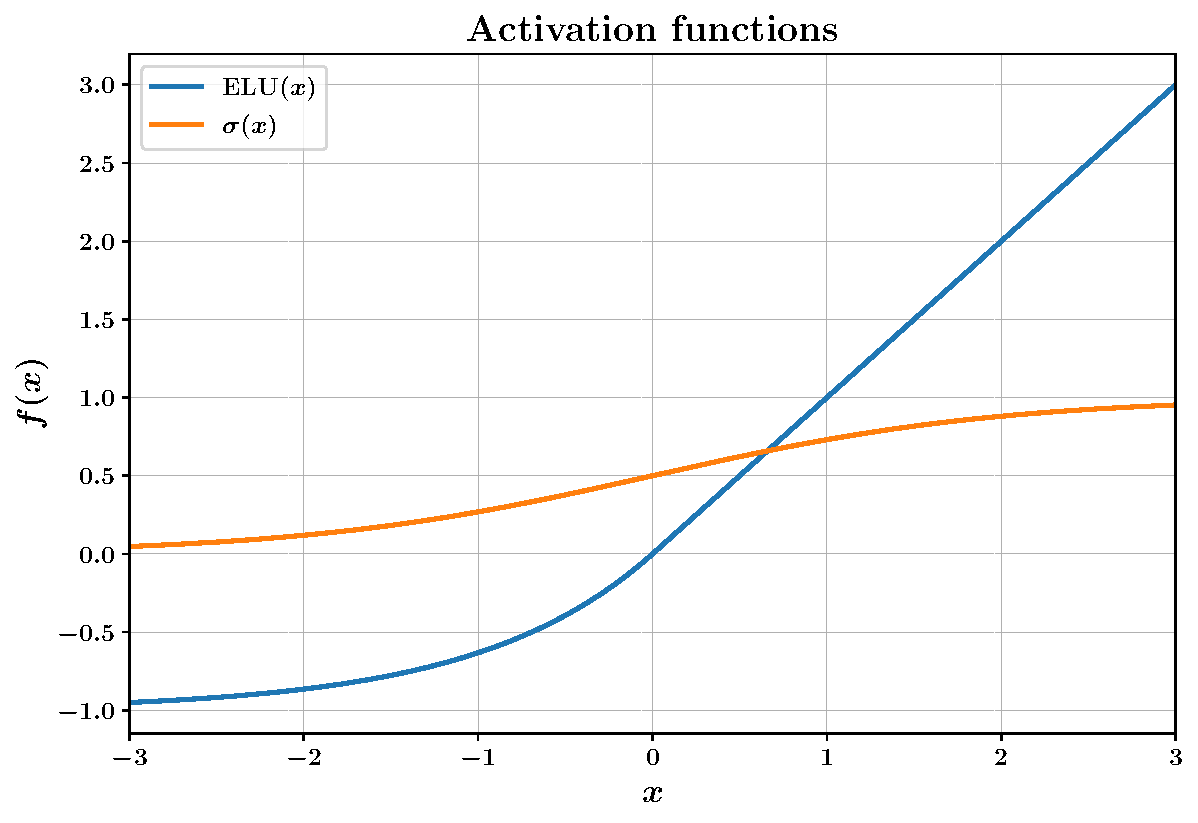
\includegraphics[height=5.8cm]{images/theory/activations/activations.pdf}
            \label{fig:theory_advanced_activations_plot}
        }
    \end{minipage}%
    \begin{minipage}[c]{0.50\linewidth}
        \vspace{0pt}
        \centering
        \subfloat[Derivatives of activation functions]{
            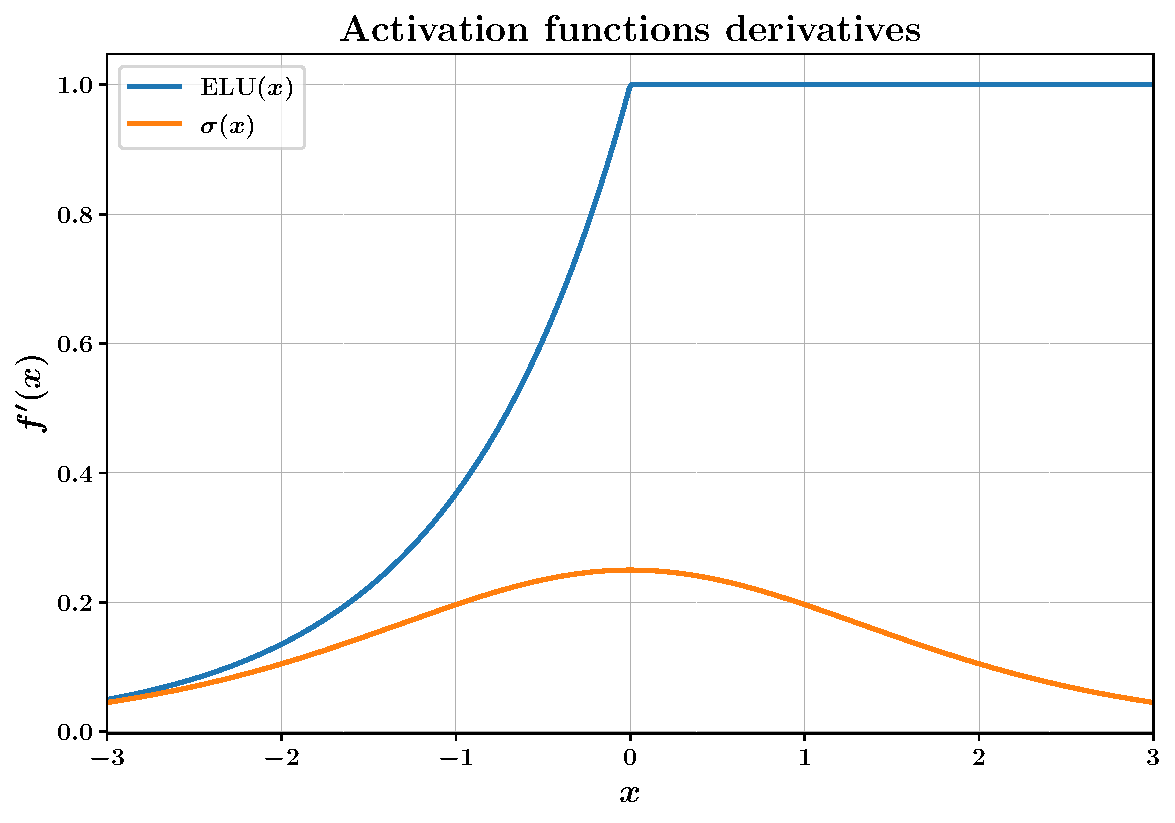
\includegraphics[height=5.8cm]{images/theory/activations/derivatives.pdf}
            \label{fig:theory_advanced_activations_derivatives}
        }
    \end{minipage}%
    \caption{Comparison between ELU and sigmoid activation functions in \textbf{\ref{fig:theory_advanced_activations_plot}}, and between their derivatives, in \textbf{\ref{fig:theory_advanced_activations_derivatives}}, which are used also for loss function gradient calculation.}
    \label{fig:theory_advanced_activation}
\end{figure*}


\paragraph{Kernel regularisation}
In general, a regularisation is any modification we make to a learning algorithm that is intended to reduce its generalization error but not its training error. In practice, the most common way to regularise a model like \( f(x;w) \) is to add a penalty for large weights to the loss function. Keeping them small often leads to more stable and general solutions and allows to train the model for a longer number of epochs before it starts to overfit. An example is the \( \ell_{2} \) regularisation, which leads to the minimisation of:
\begin{equation}
    J(y_{\mathrm{true}}, y_{\mathrm{pred}})
    =
    L(y_{\mathrm{true}}, y_{\mathrm{pred}})
    +
    \lambda \sum_{i=1}^{n_{\text{weights}}} \abs{w_{i}}^{2}
    \quad ,
\end{equation}
where \( \lambda \) is a parameter that increases or reduces the relevance of the penalty depending on its magnitude.


\paragraph{Batch normalisation}
Training networks with multiple layers can be more or less challenging. In fact, the model is updated layer-by-layer backward from the output to the input using an estimate of error that assumes the weights in the layers prior to the current layer are fixed. Because all layers are changed during an update, the update procedure is forever chasing a moving target. Batch normalization provides an elegant way of reparameterising almost any Deep Network. The reparameterisation significantly reduces the problem of coordinating updates across many layers and, so, it significantly speed up the training.

Batch normalization can be implemented during training by calculating the mean and standard deviation of the output of each layer, before applying the activation, for every batch of the training dataset. Using these statistics it is possible to perform a standardisation inside the network at the output of each layer.

\end{document}